\definecolor{bg}{rgb}{0.97,0.97,0.98}
\renewcommand{\listingscaption}{Source Code}
\newenvironment{code}{\captionsetup{type=listing}}{}
\section*{Appendix}

\begin{figure}[htp]
    \begin{subfigure}{\textwidth}  
        \centering
        \includegraphics[width=\textwidth]{5days/air-8-4-1/train_proc.png}
        \caption{The training process of each cross-valiation iteration: x-axis is $t$ value, y-axis is the evaluation result (MAE), 
        and each blue dot is an particle at time $t$ with its MAE.}
        \label{fig:2a}
    \end{subfigure}
    \begin{subfigure}{\textwidth}  
        \centering
        \includegraphics[scale=0.3]{5days/air-8-4-1/mae.png}
        \caption{The best particle from each cross-validation iteration MAE on training set (blue) and validation set (red).}
        \label{fig:2b}
    \end{subfigure}
    \caption{Training result of air-8-4-1 of next 5 days dataset with 63.233 seconds used for training.}
    \label{fig:2}
\end{figure}
\FloatBarrier

\begin{figure}[htp]
    \begin{subfigure}{\textwidth}  
        \centering
        \includegraphics[width=\textwidth]{10days/air-8-4-1/train_proc.png}
        \caption{The training process of each cross-valiation iteration: x-axis is $t$ value, y-axis is the evaluation result (MAE), 
        and each blue dot is an particle at time $t$ with its MAE.}
        \label{fig:3a}
    \end{subfigure}
    \begin{subfigure}{\textwidth}  
        \centering
        \includegraphics[scale=0.3]{10days/air-8-4-1/mae.png}
        \caption{The best particle from each cross-validation iteration MAE on training set (blue) and validation set (red).}
        \label{fig:3b}
    \end{subfigure}
    \caption{Training result of air-8-4-1 of next 10 days dataset with 61.401 seconds used for training.}
    \label{fig:3}
\end{figure}
\FloatBarrier

\begin{figure}[htp]
    \begin{subfigure}{\textwidth}  
        \centering
        \includegraphics[width=\textwidth]{5days/air-8-1-1/train_proc.png}
        \caption{The training process of each cross-valiation iteration: x-axis is $t$ value, y-axis is the evaluation result (MAE), 
        and each blue dot is an particle at time $t$ with its MAE.}
        \label{fig:4a}
    \end{subfigure}
    \begin{subfigure}{\textwidth}  
        \centering
        \includegraphics[scale=0.3]{5days/air-8-1-1/mae.png}
        \caption{The best particle from each cross-validation iteration MAE on training set (blue) and validation set (red).}
        \label{fig:4b}
    \end{subfigure}
    \caption{Training result of air-8-1-1 of next 5 days dataset with 58.504 seconds used for training.}
    \label{fig:4}
\end{figure}
\FloatBarrier

\begin{figure}[htp]
    \begin{subfigure}{\textwidth}  
        \centering
        \includegraphics[width=\textwidth]{10days/air-8-1-1/train_proc.png}
        \caption{The training process of each cross-valiation iteration: x-axis is $t$ value, y-axis is the evaluation result (MAE), 
        and each blue dot is an particle at time $t$ with its MAE.}
        \label{fig:5a}
    \end{subfigure}
    \begin{subfigure}{\textwidth}  
        \centering
        \includegraphics[scale=0.3]{10days/air-8-1-1/mae.png}
        \caption{The best particle from each cross-validation iteration MAE on training set (blue) and validation set (red).}
        \label{fig:5b}
    \end{subfigure}
    \caption{Training result of air-8-1-1 of next 10 days dataset with 53.990 seconds used for training.}
    \label{fig:5}
\end{figure}
\FloatBarrier

\begin{figure}[htp]
    \begin{subfigure}{\textwidth}  
        \centering
        \includegraphics[width=\textwidth]{5days/air-8-8-4-1/train_proc.png}
        \caption{The training process of each cross-valiation iteration: x-axis is $t$ value, y-axis is the evaluation result (MAE), 
        and each blue dot is an particle at time $t$ with its MAE.}
        \label{fig:6a}
    \end{subfigure}
    \begin{subfigure}{\textwidth}  
        \centering
        \includegraphics[scale=0.3]{5days/air-8-8-4-1/mae.png}
        \caption{The best particle from each cross-validation iteration MAE on training set (blue) and validation set (red).}
        \label{fig:6b}
    \end{subfigure}
    \caption{Training result of air-8-8-4-1 of next 5 days dataset with 81.596 seconds used for training.}
    \label{fig:6}
\end{figure}
\FloatBarrier

\begin{figure}[htp]
    \begin{subfigure}{\textwidth}  
        \centering
        \includegraphics[width=\textwidth]{10days/air-8-8-4-1/train_proc.png}
        \caption{The training process of each cross-valiation iteration: x-axis is $t$ value, y-axis is the evaluation result (MAE), 
        and each blue dot is an particle at time $t$ with its MAE.}
        \label{fig:7a}
    \end{subfigure}
    \begin{subfigure}{\textwidth}  
        \centering
        \includegraphics[scale=0.3]{10days/air-8-8-4-1/mae.png}
        \caption{The best particle from each cross-validation iteration MAE on training set (blue) and validation set (red).}
        \label{fig:7b}
    \end{subfigure}
    \caption{Training result of air-8-8-4-1 of next 10 days dataset with 78.985 seconds used for training.}
    \label{fig:7}
\end{figure}
\FloatBarrier

\begin{code}
\caption{main.rs}
\begin{minted}[fontsize=\footnotesize, bgcolor=bg, linenos]{rust}  
    pub mod activator;
    pub mod ga;
    pub mod loss;
    pub mod mlp;
    pub mod models;
    pub mod utills;
    
    use std::error::Error;
    fn main() -> Result<(), Box<dyn Error>> {
        models::airquality::air_8_4_1();
        models::airquality::air_8_1_1();
        models::airquality::air_8_8_4_1();
        Ok(())
    }
\end{minted}
\end{code}

\begin{code}
\caption{mlp.rs}
\begin{minted}[fontsize=\footnotesize, bgcolor=bg, linenos]{rust} 
use crate::activator;

#[derive(Debug)]
pub struct Layer {
    pub inputs: Vec<f64>,
    pub outputs: Vec<f64>, // need to save this for backward pass
    pub w: Vec<Vec<f64>>,
    pub b: Vec<f64>,
    pub grads: Vec<Vec<f64>>,
    pub w_prev_changes: Vec<Vec<f64>>,
    pub local_grads: Vec<f64>,
    pub b_prev_changes: Vec<f64>,
    pub act: activator::ActivationContainer,
}

impl Layer {
    pub fn new(
        input_features: u64,
        output_features: u64,
        bias: f64,
        act: activator::ActivationContainer,
    ) -> Layer {
        // initialize weights matrix
        let mut weights: Vec<Vec<f64>> = vec![];
        let mut inputs: Vec<f64> = vec![];
        let mut outputs: Vec<f64> = vec![];
        let mut grads: Vec<Vec<f64>> = vec![];
        let mut local_grads: Vec<f64> = vec![];
        let mut w_prev_changes: Vec<Vec<f64>> = vec![];
        let mut b_prev_changes: Vec<f64> = vec![];
        let mut b: Vec<f64> = vec![];

        for _ in 0..output_features {
            outputs.push(0.0);
            local_grads.push(0.0);
            b_prev_changes.push(0.0);
            b.push(bias);

            let mut w: Vec<f64> = vec![];
            let mut g: Vec<f64> = vec![];
            for _ in 0..input_features {
                if (inputs.len() as u64) < input_features {
                    inputs.push(0.0);
                }
                g.push(0.0);
                // random both positive and negative weight
                w.push(2f64 * rand::random::<f64>() - 1f64);
            }
            weights.push(w);
            grads.push(g.clone());
            w_prev_changes.push(g);
        }
        Layer {
            inputs,
            outputs,
            w: weights,
            b,
            grads,
            w_prev_changes,
            local_grads,
            b_prev_changes,
            act,
        }
    }

    pub fn forward(&mut self, inputs: &Vec<f64>) -> Vec<f64> {
        if inputs.len() != self.inputs.len() {
            panic!("forward: input size is wrong");
        }

        let result: Vec<f64> = self
            .w
            .iter()
            .zip(self.b.iter())
            .zip(self.outputs.iter_mut())
            .map(|((w_j, b_j), o_j)| {
                let sum = inputs
                    .iter()
                    .zip(w_j.iter())
                    .fold(0.0, |s, (v, w_ji)| s + w_ji * v)
                    + b_j;
                *o_j = sum;
                (self.act.func)(sum)
            })
            .collect();

        self.inputs = inputs.clone();
        result
    }

    pub fn update(&mut self, lr: f64, momentum: f64) {
        for j in 0..self.w.len() {
            let delta_b = lr * self.local_grads[j] + momentum * self.b_prev_changes[j];
            self.b[j] -= delta_b; // update each neuron bias
            self.b_prev_changes[j] = delta_b;
            for i in 0..self.w[j].len() {
                // update each weights
                let delta_w = lr * self.grads[j][i] + momentum * self.w_prev_changes[j][i];
                self.w[j][i] -= delta_w;
                self.w_prev_changes[j][i] = delta_w;
            }
        }
    }

    pub fn zero_grad(&mut self) {
        for j in 0..self.outputs.len() {
            self.local_grads[j] = 0.0;
            for i in 0..self.grads[j].len() {
                self.grads[j][i] = 0.0;
            }
        }
    }
}

#[derive(Debug)]
pub struct Net {
    pub layers: Vec<Layer>,
    pub parameters: u64,
}

impl Net {
    pub fn from_layers(layers: Vec<Layer>) -> Net {
        let mut parameters: u64 = 0;
        for l in &layers {
            parameters += (l.w.len() * l.w[0].len()) as u64;
            parameters += l.b.len() as u64;
        }

        Net { layers, parameters }
    }

    pub fn new(architecture: Vec<u64>) -> Net {
        let mut layers: Vec<Layer> = vec![];
        for i in 1..architecture.len() {
            layers.push(Layer::new(
                architecture[i - 1],
                architecture[i],
                1f64,
                activator::sigmoid(),
            ))
        }
        Net::from_layers(layers)
    }

    /// Set this network parameters from flattened parameters.
    pub fn set_params(&mut self, params: &Vec<f64>) {
        if self.parameters != params.len() as u64 {
            panic!["The neural network parameters size is not equal to individual size"];
        }
        let mut idx: usize = 0;

        for l in self.layers.iter_mut() {
            l.w.iter_mut().for_each(|w_j| {
                w_j.iter_mut().for_each(|w_ji| {
                    *w_ji = params[idx];
                    idx += 1;
                })
            });

            l.b.iter_mut().for_each(|b_i| {
                *b_i = params[idx];
                idx += 1;
            });
        }
    }

    pub fn zero_grad(&mut self) {
        for l in 0..self.layers.len() {
            self.layers[l].zero_grad();
        }
    }

    pub fn forward(&mut self, input: &Vec<f64>) -> Vec<f64> {
        let mut result = self.layers[0].forward(input);
        for l in 1..self.layers.len() {
            result = self.layers[l].forward(&result);
        }
        result
    }

    pub fn update(&mut self, lr: f64, momentum: f64) {
        for l in 0..self.layers.len() {
            self.layers[l].update(lr, momentum);
        }
    }
}

#[cfg(test)]
mod tests {
    use super::*;

    #[test]
    fn test_linear_new() {
        let linear = Layer::new(2, 3, 1.0, activator::linear());
        assert_eq!(linear.outputs.len(), 3);
        assert_eq!(linear.inputs.len(), 2);

        assert_eq!(linear.w.len(), 3);
        assert_eq!(linear.w[0].len(), 2);
        assert_eq!(linear.b.len(), 3);

        assert_eq!(linear.grads.len(), 3);
        assert_eq!(linear.w_prev_changes.len(), 3);
        assert_eq!(linear.grads[0].len(), 2);
        assert_eq!(linear.w_prev_changes[0].len(), 2);
        assert_eq!(linear.local_grads.len(), 3);
        assert_eq!(linear.b_prev_changes.len(), 3);
    }

    #[test]
    fn test_linear_forward1() {
        let mut linear = Layer::new(2, 1, 1.0, activator::sigmoid());

        for j in 0..linear.w.len() {
            for i in 0..linear.w[j].len() {
                linear.w[j][i] = 1.0;
            }
        }

        assert_eq!(linear.forward(&vec![1.0, 1.0])[0], 0.9525741268224334);
        assert_eq!(linear.outputs[0], 3.0);
    }

    #[test]
    fn test_linear_forward2() {
        let mut linear = Layer::new(2, 2, 1.0, activator::sigmoid());

        for j in 0..linear.w.len() {
            for i in 0..linear.w[j].len() {
                linear.w[j][i] = (j as f64) + 1.0;
            }
        }
        let result = linear.forward(&vec![0.0, 1.0]);
        assert_eq!(linear.outputs[0], 2.0);
        assert_eq!(linear.outputs[1], 3.0);
        assert_eq!(result[0], 0.8807970779778823);
        assert_eq!(result[1], 0.9525741268224334);
    }

    #[test]
    fn test_set_params() {
        let mut layers: Vec<Layer> = vec![];
        layers.push(Layer::new(2, 2, 1.0, activator::relu()));
        layers.push(Layer::new(2, 1, 1.0, activator::linear()));
        let mut net = Net::from_layers(layers);
        net.set_params(&vec![1.0, 1.0, 1.0, 1.0, 2.0, 2.0, 1.0, 1.0, 2.0]);

        assert_eq!(net.layers[0].w[0], vec![1.0, 1.0]);
        assert_eq!(net.layers[0].w[1], vec![1.0, 1.0]);
        assert_eq!(net.layers[0].b, vec![2.0, 2.0]);
    }
}

\end{minted}
\end{code}

\begin{code}
\caption{activator.rs}
\begin{minted}[fontsize=\footnotesize, bgcolor=bg, linenos]{rust}  
#[derive(Debug)]
pub struct ActivationContainer {
    pub func: fn(f64) -> f64,
    pub der: fn(f64) -> f64,
    pub name: String,
}

pub fn sigmoid() -> ActivationContainer {
    fn func(input: f64) -> f64 {
        1.0 / (1.0 + (-input).exp())
    }
    fn der(input: f64) -> f64 {
        func(input) * (1.0 - func(input))
    }
    ActivationContainer {
        func,
        der,
        name: "sigmoid".to_string(),
    }
}

pub fn relu() -> ActivationContainer {
    fn func(input: f64) -> f64 {
        return f64::max(0.0, input);
    }
    fn der(input: f64) -> f64 {
        if input > 0.0 {
            return 1.0;
        } else {
            return 0.0;
        }
    }
    ActivationContainer {
        func,
        der,
        name: "relu".to_string(),
    }
}

pub fn linear() -> ActivationContainer {
    fn func(input: f64) -> f64 {
        input
    }
    fn der(_input: f64) -> f64 {
        1.0
    }
    ActivationContainer {
        func,
        der,
        name: "linear".to_string(),
    }
}

#[cfg(test)]
mod tests {
    use super::*;

    #[test]
    fn test_sigmoid() {
        let act = sigmoid();

        assert_eq!((act.func)(1.0), 0.7310585786300048792512);
        assert_eq!((act.func)(-1.0), 0.2689414213699951207488);
        assert_eq!((act.func)(0.0), 0.5);
        assert_eq!((act.der)(1.0), 0.1966119332414818525374);
        assert_eq!((act.der)(-1.0), 0.1966119332414818525374);
        assert_eq!((act.der)(0.0), 0.25);
    }

    #[test]
    fn test_relu() {
        let act = relu();

        assert_eq!((act.func)(-1.0), 0.0);
        assert_eq!((act.func)(20.0), 20.0);
        assert_eq!((act.der)(-1.0), 0.0);
        assert_eq!((act.der)(20.0), 1.0);
    }
}

\end{minted}
\end{code}

\begin{code}
\caption{loss.rs}
\begin{minted}[fontsize=\footnotesize, bgcolor=bg, linenos]{rust}  
use crate::mlp;

pub struct Loss {
    outputs: Vec<f64>,
    desired: Vec<f64>,
    pub func: fn(f64, f64) -> f64,
    pub der: fn(f64, f64) -> f64,
}

impl Loss {
    /// Absolute Error
    pub fn abs_err() -> Loss {
        fn func(output: f64, desired: f64) -> f64 {
            (output - desired).abs()
        }
        fn der(output: f64, desired: f64) -> f64 {
            if output > desired {
                1.0
            } else {
                -1.0
            }
        }

        Loss {
            outputs: vec![],
            desired: vec![],
            func,
            der,
        }
    }

    /// Squared Error
    pub fn square_err() -> Loss {
        fn func(output: f64, desired: f64) -> f64 {
            0.5 * (output - desired).powi(2)
        }
        fn der(output: f64, desired: f64) -> f64 {
            output - desired
        }

        Loss {
            outputs: vec![],
            desired: vec![],
            func,
            der,
        }
    }

    /// Binary Cross Entropy
    pub fn bce() -> Loss {
        fn func(output: f64, desired: f64) -> f64 {
            -desired * output.ln() + (1.0 - desired) * (1.0 - output).ln()
        }
        fn der(output: f64, desired: f64) -> f64 {
            -(desired / output - (1.0 - desired) / (1.0 - output))
        }

        Loss {
            outputs: vec![],
            desired: vec![],
            func,
            der,
        }
    }

    pub fn criterion(&mut self, outputs: &Vec<f64>, desired: &Vec<f64>) -> f64 {
        if outputs.len() != desired.len() {
            panic!("outputs size is not equal to desired size");
        }
        let loss = outputs
            .iter()
            .zip(desired.iter())
            .fold(0.0, |ls, (o, d)| ls + (self.func)(*o, *d));
        self.outputs = outputs.clone();
        self.desired = desired.clone();
        loss
    }

    pub fn backward(&self, layers: &mut Vec<mlp::Layer>) {
        for l in (0..layers.len()).rev() {
            // output layer
            if l == layers.len() - 1 {
                for j in 0..layers[l].outputs.len() {
                    // compute grads
                    let local_grad = (self.der)(self.outputs[j], self.desired[j])
                        * (layers[l].act.der)(layers[l].outputs[j]);

                    layers[l].local_grads[j] = local_grad;

                    // set grads for each weight
                    for k in 0..(layers[l - 1].outputs.len()) {
                        layers[l].grads[j][k] =
                            (layers[l - 1].act.func)(layers[l - 1].outputs[k]) * local_grad;
                    }
                }
                continue;
            }
            // hidden layer
            for j in 0..layers[l].outputs.len() {
                // calculate local_grad based on previous local_grad
                let mut local_grad = 0f64;
                for i in 0..layers[l + 1].w.len() {
                    for k in 0..layers[l + 1].w[i].len() {
                        local_grad += layers[l + 1].w[i][k] * layers[l + 1].local_grads[i];
                    }
                }
                local_grad = (layers[l].act.der)(layers[l].outputs[j]) * local_grad;
                layers[l].local_grads[j] = local_grad;

                // set grads for each weight
                if l == 0 {
                    for k in 0..layers[l].inputs.len() {
                        layers[l].grads[j][k] = layers[l].inputs[k] * local_grad;
                    }
                } else {
                    for k in 0..layers[l - 1].outputs.len() {
                        layers[l].grads[j][k] =
                            (layers[l - 1].act.func)(layers[l - 1].outputs[k]) * local_grad;
                    }
                }
            }
        }
    }
}

#[cfg(test)]
mod tests {
    use super::*;

    #[test]
    fn test_mse_func() {
        assert_eq!((Loss::square_err().func)(2.0, 1.0), 0.5);
        assert_eq!((Loss::square_err().func)(5.0, 0.0), 12.5);
    }

    #[test]
    fn test_mse_der() {
        assert_eq!((Loss::square_err().der)(2.0, 1.0), 1.0);
        assert_eq!((Loss::square_err().der)(5.0, 0.0), 5.0);
    }

    #[test]
    fn test_mse() {
        let mut loss = Loss::square_err();

        let l = loss.criterion(&vec![2.0, 1.0, 0.0], &vec![0.0, 1.0, 2.0]);
        assert_eq!(l, 4.0);

        loss.criterion(
            &vec![34.0, 37.0, 44.0, 47.0, 48.0],
            &vec![37.0, 40.0, 46.0, 44.0, 46.0],
        );
        assert_eq!(l, 4.0);
    }

    #[test]
    fn test_bce_func() {
        println!("{}", (Loss::bce().func)(0.9, 0.0));
        println!("{}", (Loss::bce().func)(0.9, 1.0));
    }
}

\end{minted}
\end{code}

\begin{code}
\caption{models/airquality.rs}
\label{src:air}
\begin{minted}[fontsize=\footnotesize, bgcolor=bg, linenos]{rust}  
use std::time::Instant;

use crate::{
    activator, loss,
    mlp::{Layer, Net},
    swarm::{self, gen_rho},
    utills::{
        data::{self, DataSet},
        graph,
    },
};

const IMGPATH: &str = "report/assignment_4/images";

pub fn air_8_4_1() {
    fn model() -> Net {
        let mut layers: Vec<Layer> = vec![];
        layers.push(Layer::new(8, 4, 1.0, activator::relu()));
        layers.push(Layer::new(4, 1, 1.0, activator::linear()));
        Net::from_layers(layers)
    }
    air_particle_swarm(&model, "air-8-4-1");
}

pub fn air_8_1_1() {
    fn model() -> Net {
        let mut layers: Vec<Layer> = vec![];
        layers.push(Layer::new(8, 1, 1.0, activator::relu()));
        layers.push(Layer::new(1, 1, 1.0, activator::linear()));
        Net::from_layers(layers)
    }
    air_particle_swarm(&model, "air-8-1-1");
}

pub fn air_8_8_4_1() {
    fn model() -> Net {
        let mut layers: Vec<Layer> = vec![];
        layers.push(Layer::new(8, 8, 1.0, activator::relu()));
        layers.push(Layer::new(8, 4, 1.0, activator::relu()));
        layers.push(Layer::new(4, 1, 1.0, activator::linear()));
        Net::from_layers(layers)
    }
    air_particle_swarm(&model, "air-8-8-4-1");
}

pub fn validation_test(net: &mut Net, validation_set: &DataSet, training_set: &DataSet) -> (f64, f64) {
    let mut mae = 0.0;
    for data in validation_set.get_datas() {
        let result = net.forward(&data.inputs);
        let abs_err = loss::Loss::abs_err().criterion(&result, &data.labels);
        mae += abs_err;
    }
    mae = mae / validation_set.len() as f64;

    let mut t_mae = 0.0;
    for data in training_set.get_datas() {
        let result = net.forward(&data.inputs);
        let abs_err = loss::Loss::abs_err().criterion(&result, &data.labels);
        t_mae += abs_err;
    }
    (mae, t_mae/training_set.len() as f64)
}

pub fn pso_fit(model: &dyn Fn() -> Net, dataset: &DataSet, folder: String) -> f32 {
    let mut loss = loss::Loss::abs_err();
    let max_epoch = 100;
    let mut train_proc: Vec<Vec<(i32, f64)>> = (0..10).into_iter().map(|_| vec![]).collect();
    let mut valid_mae: Vec<f64> = vec![];
    let mut train_mae: Vec<f64> = vec![];

    let start = Instant::now();
    for (j, dt) in dataset.cross_valid_set(0.1).iter().enumerate() {
        let (training_set, validation_set) = dt.0.minmax_norm(&dt.1);

        let mut net = model();
        let mut groups = swarm::init_particles_group(&net, 5, 4);

        for i in 0..max_epoch {
            for (k, g) in groups.iter_mut().enumerate() {
                for (_, x) in g.particles.iter_mut().enumerate() {
                    net.set_params(&x.position);
                    let mut run_loss = 0.0;
                    for data in training_set.get_shuffled() {
                        let result = net.forward(&data.inputs);
                        run_loss += loss.criterion(&result, &data.labels);
                    }
                    let mae = run_loss / training_set.len() as f64; // Mean Absolute Error, F(x_i(t))
                    if mae < x.f {
                        x.f = mae;
                        x.best_pos = x.position.clone();
                    }
                    if mae < g.lbest_f {
                        g.lbest_f = mae; // set gbest
                        g.lbest_pos = x.position.clone();
                    }
                    x.update_speed(&g.lbest_pos, gen_rho(1.0), gen_rho(1.5));
                    x.change_pos();
                    train_proc[j].push((i, x.f));
                }
                println!("{}, {} lbest : {:.5e}", k, i, g.lbest_f);
            }
        }

        let best_group = &groups
            .iter()
            .reduce(|best, x| if best.lbest_f < x.lbest_f { best } else { x })
            .unwrap();

        let gbest = best_group
            .particles
            .iter()
            .reduce(|best, ind| if best.f < ind.f { best } else { ind })
            .unwrap();

        net.set_params(&gbest.best_pos);
        //io::save(&net.layers, "models/air/air-8-4-1.json".into()).unwrap();
        let (v_mae, t_mae) = validation_test(&mut net, &validation_set, &training_set);   
        valid_mae.push(v_mae);
        train_mae.push(t_mae);
    }

    let duration = start.elapsed();
    
    graph::draw_ga_progress(
        &train_proc,
        format!("{}/{}/train_proc.png", IMGPATH, folder),
        12.0,
    )
    .unwrap();

    graph::hist::draw_2hist(
        [&valid_mae, &train_mae],
        "Validation/Training MAE",
        ("Iteration", "Validation/Training MAE"),
        format!("{}/{}/mae.png", IMGPATH, folder),
    ).unwrap();

    duration.as_secs_f32()
}

pub fn air_particle_swarm(model: &dyn Fn() -> Net, folder: &str) {
    let (dataset_five, dataset_ten) =
        data::airquality_dataset().expect("Something wrong with airquality_dataset");

    let t1 = pso_fit(model, &dataset_five, format!("5days/{}", folder));
    let t2 = pso_fit(model, &dataset_ten, format!("10days/{}", folder));

    println!("t1: {:.3} sec, t2: {:.3} sec", t1, t2);
}


\end{minted}
\end{code}

\begin{code}
\caption{swarm/mod.rs}
\label{src:swarm}
\begin{minted}[fontsize=\footnotesize, bgcolor=bg, linenos]{rust} 
use rand::{distributions::Uniform, prelude::Distribution};

use crate::mlp::Net;

#[derive(Debug, Clone)]
pub struct Individual {
    pub best_pos: Vec<f64>,
    pub position: Vec<f64>,
    pub f: f64, // evaluation of this individual
    pub speed: Vec<f64>,
}

impl Individual {
    pub fn new(position: Vec<f64>) -> Individual {
        let mut rand = rand::thread_rng();
        let dist = Uniform::from(-1.0..=1.0);
        let speed: Vec<f64> = position.iter().map(|_i| dist.sample(&mut rand)).collect();
        Individual {
            best_pos: position.clone(),
            position,
            f: f64::MAX,
            speed,
        }
    }

    /// Individual best speed updater
    pub fn ind_update_speed(&mut self, rho: f64) {
        self.speed
            .iter_mut()
            .zip(self.best_pos.iter().zip(self.position.iter()))
            .for_each(|(v, (x_b, x))| {
                *v = *v + rho * (*x_b - *x);
            });
    }

    /// Speed updator with social component included
    pub fn update_speed(&mut self, other_best: &Vec<f64>, rho1: f64, rho2: f64) {
        let w = 1.0;
        self.speed
            .iter_mut()
            .zip(
                self.position
                    .iter()
                    .zip(self.best_pos.iter().zip(other_best.iter())),
            )
            .for_each(|(v, (x, (x_b, x_gb)))| {
                *v = w * *v + rho1 * (*x_b - *x) + rho2 * (*x_gb - *x);
            });
    }

    pub fn change_pos(&mut self) {
        self.position
            .iter_mut()
            .zip(self.speed.iter())
            .for_each(|(x, v)| {
                *x = *x + v;
            });
    }
}

pub fn gen_rho(c: f64) -> f64 {
    let mut rand = rand::thread_rng();
    let dist = Uniform::from(0.0..=1.0);
    dist.sample(&mut rand) * c
}

/// Create inital particles of MLP from layers
///
/// return: particles
pub fn init_particles(net: &Net, amount: u32) -> Vec<Individual> {
    let mut inidividuals: Vec<Individual> = vec![];
    for _ in 0..amount {
        let mut position: Vec<f64> = Vec::with_capacity(net.parameters as usize);
        for l in net.layers.iter() {
            for output in l.w.iter() {
                for _ in output.iter() {
                    // new random weight in range [-1, 1]
                    position.push(2f64 * rand::random::<f64>() - 1f64);
                }
            }
            for bias in l.b.iter() {
                position.push(*bias);
            }
        }
        inidividuals.push(Individual::new(position));
    }
    inidividuals
}

pub struct IndividualGroup {
    pub particles: Vec<Individual>,
    pub lbest_f: f64,
    pub lbest_pos: Vec<f64>,
}

impl IndividualGroup {
    pub fn add(&mut self, individual: Individual) {
        self.particles.push(individual);
    }
}

pub fn init_particles_group(net: &Net, group: usize, group_size: u32) -> Vec<IndividualGroup> {
    (0..group)
        .into_iter()
        .map(|_| {
            let particles = init_particles(&net, group_size + 1);
            IndividualGroup {
                particles: particles[1..].into(),
                lbest_f: f64::MAX,
                lbest_pos: particles[0].position.clone(),
            }
        })
        .collect()
}

#[cfg(test)]
mod tests {
    use crate::{activator, mlp::Layer};

    use super::*;

    #[test]
    fn test_update_speed() {
        fn f(pos: &Vec<f64>) -> f64 {
            pos[0].powi(2) + 2.0 * pos[1]
        }

        let mut p1 = Individual::new(vec![1.0, 1.0]);
        p1.f = 4.0;
        p1.speed = vec![0.5, 0.5];

        let gbest = vec![0.5, 1.0];

        // trainning
        let eval_result = f(&p1.position);
        if eval_result < p1.f {
            p1.f = eval_result;
            p1.best_pos = p1.position.clone();
        }

        p1.update_speed(&gbest, 1.0, 1.0);
        p1.change_pos();

        assert_eq!(p1.speed, vec![0.0, 0.5]);
        assert_eq!(p1.position, vec![1.0, 1.5]);
    }

    #[test]
    fn test_split() {
        let mut layers: Vec<Layer> = vec![];
        layers.push(Layer::new(4, 2, 1.0, activator::sigmoid()));
        layers.push(Layer::new(2, 1, 1.0, activator::sigmoid()));
        let net = Net::from_layers(layers);

        let groups = init_particles_group(&net, 3, 3);
        assert_eq!(groups.len(), 3);
        assert_eq!(groups[2].particles.len(), 3);

        let groups = init_particles_group(&net, 2, 5);
        assert_eq!(groups.len(), 2);
        assert_eq!(groups[0].particles.len(), 5);
    }
}

\end{minted}
\end{code}

\begin{code}
\caption{utills/data.rs}
\label{src:data}
\begin{minted}[fontsize=\footnotesize, bgcolor=bg, linenos]{rust}  
use super::io::read_lines;
use chrono::{DateTime, Duration, TimeZone, Utc};
use rand::prelude::SliceRandom;
use serde::Deserialize;
use std::error::Error;

pub fn max(vec: &Vec<f64>) -> f64 {
    vec.iter().fold(f64::NAN, |max, &v| v.max(max))
}

pub fn min(vec: &Vec<f64>) -> f64 {
    vec.iter().fold(f64::NAN, |min, &v| v.min(min))
}

pub fn std(vec: &Vec<f64>, mean: f64) -> f64 {
    let n = vec.len() as f64;
    vec.iter()
        .fold(0.0f64, |sum, &val| sum + (val - mean).powi(2) / n)
        .sqrt()
}

pub fn mean(vec: &Vec<f64>) -> f64 {
    let n = vec.len() as f64;
    vec.iter().fold(0.0f64, |mean, &val| mean + val / n)
}

pub fn standardization(data: &Vec<f64>, mean: f64, std: f64) -> Vec<f64> {
    data.iter().map(|x| (x - mean) / std).collect()
}

pub fn minmax_norm(data: &Vec<f64>, min: f64, max: f64) -> Vec<f64> {
    data.iter().map(|x| (x - min) / (max - min)).collect()
}

#[derive(Debug, Clone)]
pub struct Data {
    pub inputs: Vec<f64>,
    pub labels: Vec<f64>,
}
#[derive(Clone)]
pub struct DataSet {
    datas: Vec<Data>,
}

impl DataSet {
    pub fn new(datas: Vec<Data>) -> DataSet {
        DataSet { datas }
    }

    pub fn cross_valid_set(&self, percent: f64) -> Vec<(DataSet, DataSet)> {
        if percent < 0.0 && percent > 1.0 {
            panic!("argument percent must be in range [0, 1]")
        }
        let k = (percent * (self.datas.len() as f64)).ceil() as usize; // fold size
        let n = (self.datas.len() as f64 / k as f64).ceil() as usize; // number of folds
        let datas = self.get_shuffled().clone(); // shuffled data before slicing it
        let mut set: Vec<(DataSet, DataSet)> = vec![];

        let mut curr: usize = 0;
        for _ in 0..n {
            let r_pt: usize = if curr + k > datas.len() {
                datas.len()
            } else {
                curr + k
            };

            let validation_set: Vec<Data> = datas[curr..r_pt].to_vec();
            let training_set: Vec<Data> = if curr > 0 {
                let mut temp = datas[0..curr].to_vec();
                temp.append(&mut datas[r_pt..datas.len()].to_vec());
                temp
            } else {
                datas[r_pt..datas.len()].to_vec()
            };

            set.push((DataSet::new(training_set), DataSet::new(validation_set)));
            curr += k
        }
        set
    }

    pub fn data_points(&self) -> Vec<f64> {
        let mut data_points: Vec<f64> = vec![];
        for mut dt in self.datas.clone() {
            data_points.append(&mut dt.inputs);
            data_points.append(&mut dt.labels);
        }
        data_points
    }

    pub fn len(&self) -> usize {
        self.datas.len()
    }

    pub fn standardization(&self, valid_set: &DataSet) -> (DataSet, DataSet) {
        let size = self.datas[0].inputs.len();
        let features: Vec<(Vec<f64>, Vec<f64>)> = (0..size)
            .into_iter()
            .map(|i| {
                let feature = self.get_feature(i);
                let v_feature = valid_set.get_feature(i);
                let mean = mean(&feature);
                let std = std(&feature, mean);
                (
                    standardization(&feature, mean, std),
                    standardization(&v_feature, mean, std),
                )
            })
            .collect();

        let datas: Vec<Data> = self
            .datas
            .iter()
            .enumerate()
            .map(|(i, dt)| Data {
                labels: dt.labels.clone(),
                inputs: features.iter().map(|x| x.0[i]).collect(),
            })
            .collect();

        let v_datas: Vec<Data> = valid_set
            .datas
            .iter()
            .enumerate()
            .map(|(i, dt)| Data {
                labels: dt.labels.clone(),
                inputs: features.iter().map(|x| x.1[i]).collect(),
            })
            .collect();

        (DataSet::new(datas), DataSet::new(v_datas))
    }

    pub fn minmax_norm(&self, valid_set: &DataSet) -> (DataSet, DataSet) {
        let size = self.datas[0].inputs.len();
        let features: Vec<(Vec<f64>, Vec<f64>)> = (0..size)
            .into_iter()
            .map(|i| {
                let feature = self.get_feature(i);
                let v_feature = valid_set.get_feature(i);
                let min = min(&feature);
                let max = max(&feature);
                (
                    minmax_norm(&feature, min, max),
                    minmax_norm(&v_feature, min, max),
                )
            })
            .collect();

        let datas: Vec<Data> = self
            .datas
            .iter()
            .enumerate()
            .map(|(i, dt)| Data {
                labels: dt.labels.clone(),
                inputs: features.iter().map(|x| x.0[i]).collect(),
            })
            .collect();

        let v_datas: Vec<Data> = valid_set
            .datas
            .iter()
            .enumerate()
            .map(|(i, dt)| Data {
                labels: dt.labels.clone(),
                inputs: features.iter().map(|x| x.1[i]).collect(),
            })
            .collect();

        (DataSet::new(datas), DataSet::new(v_datas))
    }

    pub fn get_datas(&self) -> Vec<Data> {
        self.datas.clone()
    }

    pub fn get_feature(&self, i: usize) -> Vec<f64> {
        if i >= self.datas[0].inputs.len() {
            panic!("i should not exceed inputs feature size");
        }

        self.datas.iter().map(|data| data.inputs[i]).collect()
    }

    pub fn get_label(&self, i: usize) -> Vec<f64> {
        if i >= self.datas[0].labels.len() {
            panic!("i should not exceed inputs feature size");
        }

        self.datas.iter().map(|data| data.labels[i]).collect()
    }

    pub fn get_shuffled(&self) -> Vec<Data> {
        let mut shuffled_datas = self.datas.clone();
        shuffled_datas.shuffle(&mut rand::thread_rng());
        shuffled_datas
    }
}

pub fn confusion_count(
    matrix: &mut [[i32; 2]; 2],
    result: &Vec<f64>,
    label: &Vec<f64>,
    threshold: f64,
) {
    if result[0] > threshold {
        // true positive
        if label[0] == 1.0 {
            matrix[0][0] += 1
        } else {
            // false negative
            matrix[1][0] += 1
        }
    } else if result[0] <= threshold {
        // true negative
        if label[0] == 0.0 {
            matrix[1][1] += 1
        }
        // false positive
        else {
            matrix[0][1] += 1
        }
    }
}

pub fn un_standardization(value: f64, mean: f64, std: f64) -> f64 {
    value * std + mean
}

pub fn xor_dataset() -> DataSet {
    let inputs = vec![[0.0, 0.0], [0.0, 1.0], [1.0, 0.0], [1.0, 1.0]];
    let labels = vec![[0.0], [1.0], [1.0], [0.0]];
    let mut datas: Vec<Data> = vec![];
    for i in 0..4 {
        datas.push(Data {
            inputs: inputs[i].to_vec(),
            labels: labels[i].to_vec(),
        });
    }

    DataSet::new(datas)
}

pub fn flood_dataset() -> Result<DataSet, Box<dyn Error>> {
    #[derive(Deserialize)]
    struct Record {
        s1_t3: f64,
        s1_t2: f64,
        s1_t1: f64,
        s1_t0: f64,
        s2_t3: f64,
        s2_t2: f64,
        s2_t1: f64,
        s2_t0: f64,
        t7: f64,
    }

    let mut datas: Vec<Data> = vec![];
    let mut reader = csv::Reader::from_path("data/flood_dataset.csv")?;
    for record in reader.deserialize() {
        let record: Record = record?;
        let mut inputs: Vec<f64> = vec![];
        // station 1
        inputs.push(record.s1_t3);
        inputs.push(record.s1_t2);
        inputs.push(record.s1_t1);
        inputs.push(record.s1_t0);
        // station 2
        inputs.push(record.s2_t3);
        inputs.push(record.s2_t2);
        inputs.push(record.s2_t1);
        inputs.push(record.s2_t0);

        let labels: Vec<f64> = vec![f64::from(record.t7)];
        datas.push(Data { inputs, labels });
    }
    Ok(DataSet::new(datas))
}

pub fn cross_dataset() -> Result<DataSet, Box<dyn Error>> {
    let mut datas: Vec<Data> = vec![];
    let mut lines = read_lines("data/cross.pat")?;
    while let (Some(_), Some(Ok(l1)), Some(Ok(l2))) = (lines.next(), lines.next(), lines.next()) {
        let mut inputs: Vec<f64> = vec![];
        let mut labels: Vec<f64> = vec![];
        for w in l1.split(" ") {
            let v: f64 = w.parse().unwrap();
            inputs.push(v);
        }
        for w in l2.split(" ") {
            let v: f64 = w.parse().unwrap();
            // class 1 0 -> 1
            // class 0 1 -> 0
            labels.push(v);
            break;
        }
        datas.push(Data { inputs, labels });
    }
    Ok(DataSet::new(datas))
}

pub fn wdbc_dataset() -> Result<DataSet, Box<dyn Error>> {
    let mut datas: Vec<Data> = vec![];
    let mut lines = read_lines("data/wdbc.txt")?;
    while let Some(Ok(line)) = lines.next() {
        let mut inputs: Vec<f64> = vec![];
        let mut labels: Vec<f64> = vec![]; // M (malignant) = 1.0, B (benign) = 0.0
        let arr: Vec<&str> = line.split(",").collect();
        if arr[1] == "M" {
            labels.push(1.0);
        } else if arr[1] == "B" {
            labels.push(0.0);
        }
        for w in &arr[2..] {
            let v: f64 = w.parse()?;
            inputs.push(v);
        }
        datas.push(Data { inputs, labels });
    }
    Ok(DataSet::new(datas))
}

/// Return `(desired = next five days, desired = next ten days)`
pub fn airquality_dataset() -> Result<(DataSet, DataSet), Box<dyn Error>> {
    // nx is not used
    #[derive(Deserialize, Debug)]
    struct Record {
        #[serde(rename = "Date")]
        date: String,
        #[serde(rename = "Time")]
        time: String,
        #[serde(rename = "PT08.S1(CO)")]
        pt_s1: i32,
        #[serde(rename = "C6H6(GT)")]
        benzene: f64,
        #[serde(rename = "PT08.S2(NMHC)")]
        pt_s2: i32,
        #[serde(rename = "PT08.S3(NOx)")]
        pt_s3: i32,
        #[serde(rename = "PT08.S4(NO2)")]
        pt_s4: i32,
        #[serde(rename = "PT08.S5(O3)")]
        pt_s5: i32,
        #[serde(rename = "T")]
        temp: f64,
        #[serde(rename = "RH")]
        rh: f64,
        #[serde(rename = "AH")]
        ah: f64,
    }
    #[derive(Debug)]
    struct RecData {
        datetime: DateTime<Utc>,
        input: Vec<f64>,
        output: Vec<f64>,
        pub okay: bool,
    }
    /// add to input if input is true else add to output
    fn rec_add(recdata: &mut RecData, v: f64, input: bool) {
        if v == -200.0 {
            recdata.okay = false;
        }
        if input {
            recdata.input.push(v);
        } else {
            recdata.output.push(v)
        };
    }

    impl RecData {
        pub fn new(record: &Record) -> RecData {
            let datetime_str = format!("{} {}", record.date, record.time);
            let datetime = Utc
                .datetime_from_str(&datetime_str, "%-m/%-d/%Y %-H:%M:%S")
                .unwrap();

            let mut recdata = RecData {
                datetime,
                input: vec![],
                output: vec![],
                okay: true,
            };
            rec_add(&mut recdata, record.pt_s1 as f64, true);
            rec_add(&mut recdata, record.pt_s2 as f64, true);
            rec_add(&mut recdata, record.pt_s3 as f64, true);
            rec_add(&mut recdata, record.pt_s4 as f64, true);
            rec_add(&mut recdata, record.pt_s5 as f64, true);
            rec_add(&mut recdata, record.temp, true);
            rec_add(&mut recdata, record.rh, true);
            rec_add(&mut recdata, record.ah, true);
            rec_add(&mut recdata, record.benzene, false);
            recdata
        }
    }

    let mut reader = csv::Reader::from_path("data/AirQualityUCI.csv")?;
    let mut rec_datas: Vec<RecData> = vec![];
    for record in reader.deserialize() {
        let rec_data = RecData::new(&record.unwrap());
        if rec_data.okay {
            rec_datas.push(rec_data)
        };
    }

    //  Duration::days(5)
    let mut datas_five: Vec<Data> = vec![];
    let mut datas_ten: Vec<Data> = vec![];

    for (i, x) in rec_datas.iter().enumerate() {
        let next_five_days = x.datetime + Duration::days(5);
        let next_ten_dats = x.datetime + Duration::days(10);

        let mut labels_five: Vec<f64> = vec![];
        let mut labels_ten: Vec<f64> = vec![];

        for y in &rec_datas[i..] {
            if y.datetime == next_five_days {
                labels_five = y.output.clone();
            }
            if y.datetime == next_ten_dats {
                labels_ten = y.output.clone();
                break;
            }
        }

        if labels_five.len() == 0 && labels_ten.len() == 0 {
            break;
        }
        if labels_five.len() != 0 {
            datas_five.push(Data {
                inputs: x.input.clone(),
                labels: labels_five,
            });
        }
        if labels_ten.len() != 0 {
            datas_ten.push(Data {
                inputs: x.input.clone(),
                labels: labels_ten,
            });
        }
    }
    Ok((DataSet::new(datas_five), DataSet::new(datas_ten)))
}

#[cfg(test)]
mod tests {
    use super::*;

    #[test]
    fn test_airquality() -> Result<(), Box<dyn Error>> {
        let (dt5, _) = airquality_dataset().unwrap();

        let dt = &dt5.cross_valid_set(0.1)[0];
        let (train, _) = dt.0.minmax_norm(&dt.1);

        for dt in train.get_datas().iter() {
            for v in dt.inputs.iter() {
                print!("{:.3e} ", v);
            }
            print!("{:.3e}\n", dt.labels[0]);
        }
        println!("{}", train.len());
        Ok(())
    }

    #[test]
    fn test_minmax_norm() {
        let datas: Vec<Data> = (0..=10)
            .into_iter()
            .map(|i| Data {
                labels: vec![0.0],
                inputs: vec![i as f64 * 10.0],
            })
            .collect();
        let v_datas: Vec<Data> = (0..=10)
            .into_iter()
            .map(|i| Data {
                labels: vec![0.0],
                inputs: vec![i as f64 * 5.0],
            })
            .collect();

        let (t, v) = DataSet::new(datas).minmax_norm(&DataSet::new(v_datas));

        let expected = vec![0.0, 0.1, 0.2, 0.3, 0.4, 0.5, 0.6, 0.7, 0.8, 0.9, 1.0];
        for (i, x) in t.get_feature(0).iter().enumerate() {
            assert_eq!(*x, expected[i]);
        }
        let v_expected = vec![
            0.0, 0.05, 0.10, 0.15, 0.20, 0.25, 0.30, 0.35, 0.40, 0.45, 0.50,
        ];
        for (i, x) in v.get_feature(0).iter().enumerate() {
            assert_eq!(*x, v_expected[i])
        }
    }
}

\end{minted}
\end{code}

\begin{code}
\caption{utills/graph/mod.rs}
\begin{minted}[fontsize=\footnotesize, bgcolor=bg, linenos]{rust}  
use plotters::coord::Shift;
use plotters::prelude::*;
use std::error::Error;

pub mod hist;

const FONT: &str = "Roboto Mono";
const CAPTION: i32 = 70;
const SERIE_LABEL: i32 = 32;
const AXIS_LABEL: i32 = 40;

pub struct LossGraph {
    loss: Vec<Vec<f64>>,
    valid_loss: Vec<Vec<f64>>,
}

impl LossGraph {
    pub fn new() -> LossGraph {
        let loss: Vec<Vec<f64>> = vec![];
        let valid_loss: Vec<Vec<f64>> = vec![];
        LossGraph { loss, valid_loss }
    }

    pub fn add_loss(&mut self, training: Vec<f64>, validation: Vec<f64>) {
        self.loss.push(training);
        self.valid_loss.push(validation);
    }
    /// Draw training loss and validation loss at each epoch (x_vec)
    pub fn draw_loss(
        &self,
        idx: u32,
        root: &DrawingArea<BitMapBackend, Shift>,
        loss_vec: &Vec<f64>,
        valid_loss_vec: &Vec<f64>,
        max_loss: f64,
    ) -> Result<(), Box<dyn Error>> {
        let min_loss1 = loss_vec.iter().fold(f64::NAN, |min, &val| val.min(min));
        let min_loss2 = valid_loss_vec
            .iter()
            .fold(f64::NAN, |min, &val| val.min(min));
        let min_loss = if min_loss1.min(min_loss2) > 0.0 {
            0.0
        } else {
            min_loss1.min(min_loss2)
        };

        let mut chart = ChartBuilder::on(&root)
            .caption(
                format!("Loss {}", idx),
                ("Hack", 44, FontStyle::Bold).into_font(),
            )
            .margin(20)
            .x_label_area_size(50)
            .y_label_area_size(60)
            .build_cartesian_2d(0..loss_vec.len(), min_loss..max_loss)?;

        chart
            .configure_mesh()
            .y_desc("Loss")
            .x_desc("Epochs")
            .axis_desc_style(("Hack", 20))
            .draw()?;

        chart.draw_series(LineSeries::new(
            loss_vec.iter().enumerate().map(|(i, x)| (i + 1, *x)),
            &RED,
        ))?;

        chart.draw_series(LineSeries::new(
            valid_loss_vec.iter().enumerate().map(|(i, x)| (i + 1, *x)),
            &BLUE,
        ))?;

        root.present()?;
        Ok(())
    }

    pub fn max_loss(&self) -> f64 {
        f64::max(
            self.loss.iter().fold(f64::NAN, |max, vec| {
                let max_loss = vec.iter().fold(f64::NAN, |max, &val| val.max(max));
                f64::max(max_loss, max)
            }),
            self.valid_loss.iter().fold(f64::NAN, |max, vec| {
                let max_loss = vec.iter().fold(f64::NAN, |max, &val| val.max(max));
                f64::max(max_loss, max)
            }),
        )
    }

    pub fn draw(&self, path: String) -> Result<(), Box<dyn Error>> {
        let root = BitMapBackend::new(&path, (2000, 1000)).into_drawing_area();
        root.fill(&WHITE)?;
        // hardcode for 10 iteraions
        let drawing_areas = root.split_evenly((2, 5));

        let mut loss_iter = self.loss.iter();
        let mut valid_loss_iter = self.valid_loss.iter();
        let max_loss = self.max_loss();
        for (drawing_area, idx) in drawing_areas.iter().zip(1..) {
            if let (Some(loss_vec), Some(valid_loss_vec)) =
                (loss_iter.next(), valid_loss_iter.next())
            {
                self.draw_loss(idx, drawing_area, loss_vec, valid_loss_vec, max_loss)?;
            }
        }
        Ok(())
    }
}

/// Draw confusion matrix
pub fn draw_confustion(matrix_vec: Vec<[[i32; 2]; 2]>, path: String) -> Result<(), Box<dyn Error>> {
    let root = BitMapBackend::new(&path, (2000, 1100)).into_drawing_area();
    root.fill(&WHITE)?;

    let (top, down) = root.split_vertically(1000);

    let mut chart = ChartBuilder::on(&down)
        .margin(20)
        .margin_left(40)
        .margin_right(40)
        .x_label_area_size(40)
        .build_cartesian_2d(0i32..50i32, 0i32..1i32)?;
    chart
        .configure_mesh()
        .disable_y_axis()
        .disable_y_mesh()
        .x_labels(3)
        .label_style((FONT, 40))
        .draw()?;

    chart.draw_series((0..50).map(|x| {
        Rectangle::new(
            [(x, 0), (x + 1, 1)],
            HSLColor(
                240.0 / 360.0 - 240.0 / 360.0 * (x as f64 / 50.0),
                0.7,
                0.1 + 0.4 * x as f64 / 50.0,
            )
            .filled(),
        )
    }))?;
    // hardcode for 10 iteraions
    let drawing_areas = top.split_evenly((2, 5));
    let mut matrix_iter = matrix_vec.iter();
    for (drawing_area, idx) in drawing_areas.iter().zip(1..) {
        if let Some(matrix) = matrix_iter.next() {
            let mut chart = ChartBuilder::on(&drawing_area)
                .caption(
                    format!("Iteration {}", idx),
                    (FONT, 40, FontStyle::Bold).into_font(),
                )
                .margin(20)
                .build_cartesian_2d(0i32..2i32, 2i32..0i32)?
                .set_secondary_coord(0f64..2f64, 2f64..0f64);

            chart
                .configure_mesh()
                .disable_axes()
                .max_light_lines(4)
                .disable_x_mesh()
                .disable_y_mesh()
                .label_style(("Hack", 20))
                .draw()?;

            chart.draw_series(
                matrix
                    .iter()
                    .zip(0..)
                    .map(|(l, y)| l.iter().zip(0..).map(move |(v, x)| (x, y, v)))
                    .flatten()
                    .map(|(x, y, v)| {
                        Rectangle::new(
                            [(x, y), (x + 1, y + 1)],
                            HSLColor(
                                240.0 / 360.0 - 240.0 / 360.0 * (*v as f64 / 50.0),
                                0.7,
                                0.1 + 0.4 * *v as f64 / 50.0,
                            )
                            .filled(),
                        )
                    }),
            )?;

            chart.draw_secondary_series(
                matrix
                    .iter()
                    .zip(0..)
                    .map(|(l, y)| l.iter().zip(0..).map(move |(v, x)| (x, y, v)))
                    .flatten()
                    .map(|(x, y, v)| {
                        let text: String = if x == 0 && y == 0 {
                            format!["TP:{}", v]
                        } else if x == 1 && y == 0 {
                            format!["FP:{}", v]
                        } else if x == 0 && y == 1 {
                            format!["FN:{}", v]
                        } else {
                            format!["TN:{}", v]
                        };

                        Text::new(
                            text,
                            ((2.0 * x as f64 + 0.7) / 2.0, (2.0 * y as f64 + 1.0) / 2.0),
                            FONT.into_font().resize(30.0).color(&WHITE),
                        )
                    }),
            )?;
        }
    }
    root.present()?;
    Ok(())
}

/// Receive each cross-validation vector of each individual fitness value.
pub fn draw_ga_progress(
    cv_fitness: &Vec<Vec<(i32, f64)>>,
    path: String,
    max_y: f64,
) -> Result<(), Box<dyn Error>> {
    let root = BitMapBackend::new(&path, (2000, 1000)).into_drawing_area();
    root.fill(&WHITE)?;

    let max_x = cv_fitness[0]
        .iter()
        .reduce(|m, x| if m.0 > x.0 { m } else { x })
        .unwrap()
        .0;

    // This is mostly hardcoded
    let drawing_areas = root.split_evenly((2, 5));
    for ((drawing_area, idx), fitness) in drawing_areas.iter().zip(1..).zip(cv_fitness.iter()) {
        let mut chart = ChartBuilder::on(&drawing_area)
            .caption(
                format!("Iteration {}", idx),
                (FONT, 40, FontStyle::Bold).into_font(),
            )
            .margin(40)
            .x_label_area_size(20)
            .y_label_area_size(30)
            .build_cartesian_2d(0i32..max_x, 0.0..max_y)?;

        chart
            .configure_mesh()
            .x_labels(3)
            .y_labels(2)
            .label_style((FONT, 30))
            .max_light_lines(4)
            .draw()?;

        chart.draw_series(
            fitness
                .iter()
                .map(|x| Circle::new((x.0, x.1), 1, BLUE.mix(0.25).filled())),
        )?;
    }
    root.present()?;
    Ok(())
}

\end{minted}
\end{code}

\begin{code}
\caption{utills/graph/hist.rs}
\begin{minted}[fontsize=\footnotesize, bgcolor=bg, linenos]{rust}  
use plotters::prelude::*;
use std::error::Error;

use crate::utills::{graph::*, data};

pub struct Histogram2 {
    datas: [Vec<f64>; 2],
    title: String,
    axes_desc: (String, String),
}

impl Histogram2 {
    pub fn new(datas: [Vec<f64>; 2],title: &str, axes_desc: (&str, &str)) -> Histogram2 {
        Histogram2 {
            datas,
            title: title.into(),
            axes_desc: (axes_desc.0.into(), axes_desc.1.into()),
        }
    }

    pub fn mean(&self) -> Vec<f64> {
        self.datas
            .iter()
            .map(|l| {
                l.iter()
                    .fold(0f64, |mean, &val| mean + val / l.len() as f64)
            })
            .collect()
    }

    pub fn max_x(&self) -> f64 {
        self.datas
            .iter()
            .fold(0f64, |max, l| max.max(l.len() as f64))
    }

    pub fn max_y(&self) -> f64 {
        self.datas
            .iter()
            .fold(f64::MIN, |max, l| {
                let l_max = data::max(l);
                if l_max > max {
                    l_max
                }
                else {
                    max
                }
            })
    }

    pub fn draw_hist(&self, path: String, max_y: f64) -> Result<(), Box<dyn Error>> {
        let root = BitMapBackend::new(&path, (1024, 768)).into_drawing_area();
        root.fill(&WHITE)?;

        let n = self.max_x();
        let mut chart = ChartBuilder::on(&root)
            .caption(&self.title, (FONT, CAPTION, FontStyle::Bold).into_font())
            .margin(20)
            .x_label_area_size(70)
            .y_label_area_size(90)
            .build_cartesian_2d((1..n as u32).into_segmented(), 0.0..max_y)?
            .set_secondary_coord(0.0..n, 0.0..max_y);

        chart
            .configure_mesh()
            .disable_x_mesh()
            .y_max_light_lines(0)
            .y_desc(&self.axes_desc.1)
            .x_desc(&self.axes_desc.0)
            .axis_desc_style((FONT, AXIS_LABEL))
            .y_labels(3)
            .label_style((FONT, AXIS_LABEL - 10))
            .draw()?;


        let colors = [&RED, &BLUE];

        for (i, dt) in self.datas.iter().enumerate() {
            let color = colors[i % 2];
            let offset = i as f64 * 0.4;
            chart.draw_secondary_series(dt.iter().zip(0..).map(|(y, x)| {
                Rectangle::new(
                    [(x as f64 + 0.1 + offset, *y), (x as f64 + 0.5 + offset, 0f64)],
                    Into::<ShapeStyle>::into(color.mix(0.5)).filled(),
                )
            }))?;
        }

        let v: Vec<usize> = (0..(n + 1.0) as usize).collect();
        let mean = self.mean();
        for (j, m) in mean.iter().enumerate() {
            let color = colors[j % 2];
            chart
                .draw_secondary_series(LineSeries::new(
                    v.iter().map(|i| (*i as f64, *m)),
                    color.filled().stroke_width(2),
                ))?
                .label(format!("mean: {:.3}", m))
                .legend(move |(x, y)| PathElement::new(vec![(x, y), (x + 20, y)], color.filled()));
        }

        chart
            .configure_series_labels()
            .label_font((FONT, SERIE_LABEL).into_font())
            .background_style(&WHITE)
            .border_style(&BLACK)
            .draw()?;

        root.present()?;
        Ok(())
    }
}

/// Draw histogram of given datas
/// axes_desc - (for x, for y)
pub fn draw_acc_hist(
    datas: &Vec<f64>,
    title: &str,
    axes_desc: (&str, &str),
    path: String,
) -> Result<(), Box<dyn Error>> {
    let n = datas.len();
    let mean = datas
        .iter()
        .fold(0.0f64, |mean, &val| mean + val / n as f64);

    let root = BitMapBackend::new(&path, (1024, 768)).into_drawing_area();
    root.fill(&WHITE)?;

    let mut chart = ChartBuilder::on(&root)
        .caption(title, ("Hack", 44, FontStyle::Bold).into_font())
        .margin(20)
        .x_label_area_size(50)
        .y_label_area_size(60)
        .build_cartesian_2d((1..n).into_segmented(), 0.0..1.0)?
        .set_secondary_coord(1..n, 0.0..1.0);

    chart
        .configure_mesh()
        .disable_x_mesh()
        .y_max_light_lines(0)
        .y_desc(axes_desc.1)
        .x_desc(axes_desc.0)
        .axis_desc_style(("Hack", 20))
        .y_labels(3)
        .draw()?;

    let hist = Histogram::vertical(&chart)
        .style(RED.mix(0.5).filled())
        .margin(10)
        .data(datas.iter().enumerate().map(|(i, x)| (i + 1, *x)));

    chart.draw_series(hist)?;

    chart
        .draw_secondary_series(LineSeries::new(
            datas.iter().enumerate().map(|(i, _)| (i + 1, mean)),
            BLUE.filled().stroke_width(2),
        ))?
        .label(format!("mean: {:.3}", mean))
        .legend(|(x, y)| PathElement::new(vec![(x, y), (x + 20, y)], &BLUE));

    chart
        .configure_series_labels()
        .label_font(("Hack", 14).into_font())
        .background_style(&WHITE)
        .border_style(&BLACK)
        .draw()?;

    root.present()?;
    Ok(())
}

pub fn draw_acc_2hist(
    datas: [&Vec<f64>; 2],
    title: &str,
    axes_desc: (&str, &str),
    path: String,
) -> Result<(), Box<dyn Error>> {
    let hist2 = Histogram2::new([datas[0].clone(), datas[1].clone()], title, axes_desc);
    hist2.draw_hist(path, 1.0)
}

pub fn draw_2hist(
    datas: [&Vec<f64>; 2],
    title: &str,
    axes_desc: (&str, &str),
    path: String,
) -> Result<(), Box<dyn Error>> {
    let hist2 = Histogram2::new([datas[0].clone(), datas[1].clone()], title, axes_desc);
    hist2.draw_hist(path, hist2.max_y())
}


\end{minted}
\end{code}